\clearpage
{\bfseries МРНТИ 61.13.17; 31.15.27}

\section{КИНЕТИКА ТЕРМИЧЕСКОЙ ДЕСТРУКЦИИ УГЛЯ МЕСТОРОЖДЕНИЯ КИЯКТЫ}

\begin{center}
{\bfseries Н.У. Нургалиев\textsuperscript{*},} {\bfseries А.Х.Такирова, А.Ж.
Хамит, Э.Б. Жунусова, А.А. Ахаева}

Казахский университет технологии и бизнеса, г. Астана, Казахстан,

e-mail: nurgaliev\_nao@mail.ru
\end{center}

В статье проведено исследование кинетики термической деструкции угля с
использованием метода термогравиметрического анализа. Нагрев образцов
угля проводили в керамических тиглях в интервале температур 25-900 °С
при разных скоростях нагрева (3-15 град/мин) в средах азота и кислорода.
В качестве объекта исследования выбран уголь месторождения Киякты
(Казахстан). На основе построенных дифференциальных термических кривых
DTG (зависимость скорости изменения массы образца от времени) при разных
скоростях нагрева рассчитаны кинетические параметры термодеструкции
угля, с использованием уравнений неизотермической формальной кинетики.
Изучено влияние скорости и температуры нагрева угля на кинетические
параметры процесса термической деструкции органической массы угля (ОМУ).
Выявлены основные стадии разложения ОМУ. Установлено, что скорость
нагрева образцов угля заметно влияет на значения температуры и скорости
процесса, соответствующие максимумам основного разложения на
дифференциальных кривых DTG.

{\bfseries Ключевые слова:} термогравиметрический анализ, уголь,
термическая деструкция, кривые DTG, кинетические параметры, стадии
разложения, скорость нагрева.

\begin{center}
{\large\bfseries ҚИЯҚТЫ КЕН ОРЫНЫ КӨМІРНІҢ ТЕРМИЯЛЫҚ ДЕСТРУКЦИЯСЫНЫҢ КИНЕТИКАСЫ}

\vspace{1em}
{\bfseries Н.У. Нургалиев\textsuperscript{*}, А.Х.} {\bfseries Такирова, А.Ж.
Хамит, Э.Б. Жунусова, А.А.Ахаева}

Қазақ технология және бизнес университеті, Астана, Қазақстан

e-mail: nurgaliev\_nao@mail.ru
\end{center}

Мақалада термогравиметриялық анализ әдісін қолдану арқылы көмірдің
термиялық деградациясының кинетикасы зерттеу жасалған. Көмір үлгілері
қыш тигельдерде 25--900°C температура диапазонында азот пен оттегі
орталарында әртүрлі қыздыру жылдамдықтарында (3--15 град/мин)
қыздырылды. Зерттеу нысаны ретінде Қияқты кен орнының көмірі (Қазақстан)
таңдалды. Құрылған дифференциалдық қисықтар негізінде DTG (үлгі
массасының өзгеру жылдамдығының уақытқа тәуелділігі) әртүрлі қыздыру
жылдамдықтарында көмірдің термиялық деструкциясының кинетикалық
параметрлері изотермиялық емес формалды кинетика теңдеулері арқылы
есептелді. Көмірдің органикалық массасының (КОМ) термиялық бұзылу
процесінің кинетикалық параметрлеріне көмірді қыздыру жылдамдығы мен
температурасының әсері зерттелді.

КОМ ыдырауының негізгі кезеңдері анықталды. Көмір үлгілерін қыздыру
жылдамдығы DTG дифференциалды қисықтары бойынша негізгі ыдырау
максимумдарына сәйкес келетін температура мен технологиялық процестің
жылдамдығына айтарлықтай әсер ететіні анықталды.

\begin{center}
{\large\bfseries Түйінді сөздер:} термогравиметриялық талдау, көмір, термиялық
деградация, DTG қисықтары, кинетикалық параметрлер, ыдырау кезеңдері,
қыздыру жылдамдығы.

{\bfseries KINETICS OF THERMAL DESTRUCTION OF COAL FROM THE KIYAKTY
DEPOSIT}

\vspace{1em}
{\bfseries N.U. Nurgaliyev\textsuperscript{*}, A.K. Takirova, A.Z. Khamit,
E.B. Zhunussova, A.A.Akhaeva}

Kazakh University of Technology and Business, Astana, Kazakhstan,

e-mail: nurgaliev\_nao@mail.ru
\end{center}

The article studies the kinetics of thermal degradation of coal using
the method of thermogravimetric analysis. Coal samples were heated in
ceramic crucibles in the temperature range of 25-900°C at different
heating rates (3-15 deg/min) in nitrogen and oxygen media. Coal from
the Kiyakty deposit (Kazakhstan) was chosen as the object of study.
Based on the constructed differential thermal curves DTG (dependence of
the sample mass change rate on time) at different heating rates, the
kinetic parameters of thermal degradation of coal were calculated using
the equations of non-isothermal formal kinetics. The influence of the
rate and temperature of coal heating on the kinetic parameters of the
process of thermal destruction of the organic mass of coal (OMC) has
been studied. The main stages of WMD decomposition are revealed. It has
been found that the heating rate of coal samples significantly affects
the temperature and process rate corresponding to the main decomposition
maxima on the differential DTG curves.

{\bfseries Keywords:} thermogravimetric analysis, coal, thermal
degradation, DTG curves, kinetic parameters, decomposition stages,
heating rate.

\begin{multicols}{2}
{\bfseries Введение.} Для повышения экологичности и эффективности
использования твердого топлива предложены различные решения, от
газификации до оптимизации эксплуатационных параметров с применением
математического моделирования процессов деструкции. Это объясняет
повышенный интерес к исследованию кинетики процессов деструкции твердых
топлив в последнее время {[}1-4{]}. Одним из наиболее известных методов
термического анализа является метод термогравиметрического анализа
(ТГА), позволяющий исследовать основные параметры окисления твердого
топлива, в т.ч. определять кинетические параметры исследуемого процесса.

Достаточно широко распространены работы с применением ТГА {[}5-9{]},
посвященные определению констант формальной кинетики процессов конверсии
угля. Подобные работы основаны на интерпретации уравнения Аррениуса и
предположении о том, что скорость уменьшения массы твердого топлива
зависит только от температуры и степени конверсии {[}10{]}. Целью данных
работ является нахождении параметров \emph{E} и \emph{A}, называемых
энергией активации и предэкспонентой соответственно, а также
кинетической функции f(α). Вместе, эти три величины называют
кинетическим триплетом {[}11{]}.

При рассмотрении термической деструкции классическая кинетика отдельно
описывает влияние концентрации и температуры реагирующих веществ на
скорость процесса, без учета изменения концентрации в зависимости от
температуры. В неизотермической кинетике нет этого недостатка {[}12{]}.
С помощью неизотермических методов можно за относительно небольшой
промежуток времени получить важную информацию о характере протекания
процесса термодеструкции в широком температурном интервале.

Цель настоящей работы ‒ исследование зависимости скорости и температуры
нагрева угля от кинетических параметров термической деструкции ОМУ с
использованием метода ТГА. В качестве объекта исследования выбран уголь
месторождения Киякты (Казахстан). Задачами исследования является
определение основных стадий разложения ОМУ, изучение влияния скорости и
температуры нагрева угля на кинетику термодеструкции.

{\bfseries Материалы и методы.} Эксперименты по исследованию кинетики
термического разложения угля месторождения Киякты проводили на
термогравиметрическом анализаторе TGA4000 при разных скоростях нагрева в
пределах 3-15 град/мин. Использовали стандартные тестовые методы для
анализа угля согласно ASTM D7582-12 «Standard Test Methods for Proximate
Analysis of Coal and Coke by Macro Thermogravimetric Analysis».

Эксперименты на приборе ТГА проводили при двух атмосферах печи: азот и
кислород. Эксперимент проводили в два этапа. На 1-ом этапе температуру
поднимают от комнатной 25°С до 40°С и при этой температуре выдерживают
15 минут для стабилизации температуры. На втором этапе тестовый образец
в тиглях с закрытой крышкой нагревают от 40°С до 915± 3°С. При этом,
скорость нагрева при разных экспериментах устанавливают: 3, 6, 9, 12, 15
\textsuperscript{0}С/мин. При нагреве печи прибор ТГА взвешивает
закрытые тигли через определенные промежутки времени и фиксирует данные
в специальной программе. Когда для обеспечения нейтральной атмосферы
использовали азот, показатели потока сушильного газа устанавливались в
количестве от 0,4 до 1,4 от изменений объема печи за минуту. Когда в
качестве окислительного газа использовали кислород, показатели потока
устанавливались от 1,3 до 1,4 от изменений объема печи за минуту.

В данной работе расчет кинетических параметров термодеструкции ОМУ
проводили на основе уравнений неизотермической формальной кинетики в
соответствии с методикой, описанной в работе {[}13{]}.

Для характеристики исследуемого процесса выбраны следующие показатели:
потери масс угля при различных температурах; скорость
\emph{v\textsubscript{max}}, константа скорости
\emph{k\textsubscript{max}} и температура \emph{Т\textsubscript{max}},
которые соответствуют максимальной скорости потери массы (т.е.
максимумам основного разложения на кривых DTG в точках перегиба);
энергия активации \emph{E\textsubscript{акт }}и предэкспоненциальный
множитель \emph{k\textsubscript{0}}, относящиеся к стадиям основного
термического разложения угля; \emph{n -} показатель степени процесса
(безразмерная величина).

Следует отметить, что описать весь процесс деструкции угля одним
уравнением первого порядка невозможно, т.к. фактически разложение ОМУ
осуществляется при взаимодействии множества групп веществ различной
природы. Поэтому уравнениями формальной кинетики 1-го порядка можно
описать только процесс основного термического разложения ОМУ и
рассчитать кинетические параметры.

{\bfseries Результаты и обсуждение.} Характеристики угля месторождения
Киякты приведены таблице 1.
\end{multicols}

\begin{longtable}[]{@{}
  >{\raggedright\arraybackslash}p{(\columnwidth - 18\tabcolsep) * \real{0.0869}}
  >{\raggedright\arraybackslash}p{(\columnwidth - 18\tabcolsep) * \real{0.0853}}
  >{\raggedright\arraybackslash}p{(\columnwidth - 18\tabcolsep) * \real{0.1036}}
  >{\raggedright\arraybackslash}p{(\columnwidth - 18\tabcolsep) * \real{0.1036}}
  >{\raggedright\arraybackslash}p{(\columnwidth - 18\tabcolsep) * \real{0.0870}}
  >{\raggedright\arraybackslash}p{(\columnwidth - 18\tabcolsep) * \real{0.0870}}
  >{\raggedright\arraybackslash}p{(\columnwidth - 18\tabcolsep) * \real{0.0870}}
  >{\raggedright\arraybackslash}p{(\columnwidth - 18\tabcolsep) * \real{0.0978}}
  >{\raggedright\arraybackslash}p{(\columnwidth - 18\tabcolsep) * \real{0.1206}}
  >{\raggedright\arraybackslash}p{(\columnwidth - 18\tabcolsep) * \real{0.1410}}@{}}
\caption{Характеристики угля месторождения Киякты} \\
\toprule\noalign{}
\multicolumn{8}{@{}>{\raggedright\arraybackslash}p{(\columnwidth - 18\tabcolsep) * \real{0.7384} + 14\tabcolsep}}{%
\multirow{2}{*}{\begin{minipage}[b]{\linewidth}\raggedright
Cостав угля (на рабочую массу), \%
\end{minipage}}} &
\multicolumn{2}{>{\raggedright\arraybackslash}p{(\columnwidth - 18\tabcolsep) * \real{0.2616} + 2\tabcolsep}@{}}{%
\begin{minipage}[b]{\linewidth}\raggedright
Теплота сгорания,

(ккал/кг)
\end{minipage}} \\
& & & & & & & & \begin{minipage}[b]{\linewidth}\raggedright
высшая
\end{minipage} & \begin{minipage}[b]{\linewidth}\raggedright
высшая
\end{minipage} \\
\midrule\noalign{}
\endhead
\bottomrule\noalign{}
\endlastfoot
\emph{W}\textsuperscript{r} & \emph{\textsc{A}}\textsuperscript{r} &
\emph{V}\textsuperscript{daf} & \emph{C}\textsuperscript{r} &
\emph{O}\textsuperscript{r} & \emph{H}\textsuperscript{r} &
\emph{N}\textsuperscript{r} & \emph{S}\textsuperscript{r} &
\(Q_{в}^{r}\) & \(Q_{н}^{r}\) \\
9,37 & 21,25 & 43,18 & 51,56 & 13,39 & 3,26 & 0,55 & 0,62 & 4822 &
4589 \\
\end{longtable}

\begin{multicols}{2}
При анализе дифференциальных кривых DTG выявлены три стадии основного
разложения ОМУ, где наблюдаются пики с максимумами скорости потери массы
(точки перегиба). Проведем характеристики каждой из стадий на примере
среды азота.

Первая стадия с максимумом при температурах Т\textsubscript{max} в
интервале 148-229 °С обусловлена испарением влаги, улетучиванием
кислородсодержащих газов из-за распада крайних групп макромолекул. На
этой стадии осуществляется в основном частичный разрыв и отщепление
боковых цепей, обрыв связей между основными структурными звеньями,
частично удаляются сера, азот, кислород. Количество летучих веществ в
данном интервале температур невелик. На 2-й стадии наблюдается пик с
максимумом при 362-459 °С, который связан с возрастанием интенсивности
реакций термосинтеза из-за увеличения реакционной способности веществ
угля. Здесь могут осуществляться реакции расщепления гетероциклических и
оксиароматических систем, повышение количества непредельных связей, при
этом скорость образования летучих веществ возрастает.\\
3-стадия с максимумом при 478-637 °С обусловлена реакциями термораспада
наиболее термостабильных органоминеральных комплексов. К концу этой
стадии выделяется основная масса газообразных углеводородов и смольных
веществ и процесс заканчивается образованием полукокса. Дальнейшее
увеличение температуры реакции приводит к интенсификации полициклизации
и ароматизации (с выделением газообразных продуктов, в основном
водорода, и в меньшем количестве - метана, оксида углерода, азота),
происходит образование более высокомолекулярных полициклических систем
сетчатого строения {[}13{]}. При скоростях нагрева от 6 до 15 град/мин
на 3-й стадии основного разложения ОМУ пики с максимумом скорости потери
массы слабо выделяются и они уменьшаются при повышении скорости нагрева.
Это скорее всего связано с наложением ряда процессов и невозможностью их
раздельной оценки для определения кинетических характеристик.

В таблицах 2-5 приведены результаты обработки кривых DTG.
\end{multicols}


\begin{longtable}[]{@{}
  >{\raggedright\arraybackslash}p{(\columnwidth - 14\tabcolsep) * \real{0.1312}}
  >{\raggedright\arraybackslash}p{(\columnwidth - 14\tabcolsep) * \real{0.1470}}
  >{\raggedright\arraybackslash}p{(\columnwidth - 14\tabcolsep) * \real{0.1546}}
  >{\raggedright\arraybackslash}p{(\columnwidth - 14\tabcolsep) * \real{0.1546}}
  >{\raggedright\arraybackslash}p{(\columnwidth - 14\tabcolsep) * \real{0.1396}}
  >{\raggedright\arraybackslash}p{(\columnwidth - 14\tabcolsep) * \real{0.0976}}
  >{\raggedright\arraybackslash}p{(\columnwidth - 14\tabcolsep) * \real{0.0880}}
  >{\raggedright\arraybackslash}p{(\columnwidth - 14\tabcolsep) * \real{0.0874}}@{}}
\caption{Значения потери масс образцов угля и температуры
Т\textsubscript{max} на различных стадиях разложения в среде} \\
\toprule\noalign{}
\multirow{3}{*}{\begin{minipage}[b]{\linewidth}\raggedright
Скорость

нагрева,\\
°С /мин\strut
\end{minipage}} &
\multicolumn{4}{c}{Потеря массы от навески, \%} &
\multicolumn{3}{c}{Т\textsubscript{max}, °С} \\
& \multirow{2}{*}{\begin{minipage}[b]{\linewidth}\raggedright
30-300°С
\end{minipage}} &
\multirow{2}{*}{\begin{minipage}[b]{\linewidth}\raggedright
300-600°С
\end{minipage}} &
\multirow{2}{*}{\begin{minipage}[b]{\linewidth}\raggedright
600-900°С
\end{minipage}} &
\multirow{2}{*}{\begin{minipage}[b]{\linewidth}\raggedright
30-900°С
\end{minipage}} &
\multicolumn{3}{c}{Стадии разложения} \\
& & & & & \begin{minipage}[b]{\linewidth}\raggedright
1
\end{minipage} & \begin{minipage}[b]{\linewidth}\raggedright
2
\end{minipage} & \begin{minipage}[b]{\linewidth}\raggedright
3
\end{minipage} \\
\midrule\noalign{}
\endhead
\bottomrule\noalign{}
\endlastfoot
3 & 10,32 & 17,36 & 9,73 & \emph{37,41} & 148 & 362 & 478 \\
6 & 10,03 & 16,56 & 8,93 & \emph{35,52} & 176 & 403 & 527 \\
9 & 9,64 & 16,69 & 8,59 & \emph{34,92} & 193 & 425 & 562 \\
12 & 9,27 & 16,23 & 8,24 & \emph{33,74} & 205 & 441 & 603 \\
15 & 8,63 & 15,68 & 7,85 & \emph{32,16} & 229 & 459 & 637 \\
\end{longtable}

\begin{longtable}[]{@{}
  >{\raggedright\arraybackslash}p{(\columnwidth - 14\tabcolsep) * \real{0.1312}}
  >{\raggedright\arraybackslash}p{(\columnwidth - 14\tabcolsep) * \real{0.1470}}
  >{\raggedright\arraybackslash}p{(\columnwidth - 14\tabcolsep) * \real{0.1546}}
  >{\raggedright\arraybackslash}p{(\columnwidth - 14\tabcolsep) * \real{0.1546}}
  >{\raggedright\arraybackslash}p{(\columnwidth - 14\tabcolsep) * \real{0.1396}}
  >{\raggedright\arraybackslash}p{(\columnwidth - 14\tabcolsep) * \real{0.0976}}
  >{\raggedright\arraybackslash}p{(\columnwidth - 14\tabcolsep) * \real{0.0880}}
  >{\raggedright\arraybackslash}p{(\columnwidth - 14\tabcolsep) * \real{0.0874}}@{}}
\caption{Значения потери масс образцов угля и температуры
Т\textsubscript{max} на различных стадиях разложения в среде кислорода} \\
\toprule\noalign{}
\multirow{3}{*}{\begin{minipage}[b]{\linewidth}\raggedright
Скорость

нагрева,\\
°С /мин\strut
\end{minipage}} &
\multicolumn{4}{c}{Потеря массы от навески, \%} &
\multicolumn{3}{c}{Т\textsubscript{max}, °С} \\
& \multirow{2}{*}{\begin{minipage}[b]{\linewidth}\raggedright
30-300°С
\end{minipage}} &
\multirow{2}{*}{\begin{minipage}[b]{\linewidth}\raggedright
300-600°С
\end{minipage}} &
\multirow{2}{*}{\begin{minipage}[b]{\linewidth}\raggedright
600-900°С
\end{minipage}} &
\multirow{2}{*}{\begin{minipage}[b]{\linewidth}\raggedright
30-900°С
\end{minipage}} &
\multicolumn{3}{c}{Стадии разложения} \\
& & & & & \begin{minipage}[b]{\linewidth}\raggedright
1
\end{minipage} & \begin{minipage}[b]{\linewidth}\raggedright
2
\end{minipage} & \begin{minipage}[b]{\linewidth}\raggedright
3
\end{minipage} \\
\midrule\noalign{}
\endhead
\bottomrule\noalign{}
\endlastfoot
3 & 9,25 & 22,59 & 10,73 & \emph{42,57} & 154~ & 375 & 459 \\
6 & 8,23 & 21,04 & 9,88 & \emph{39,15} & 181 & 395 & 518 \\
9 & 8,01 & 20,23 & 9,57 & \emph{37,81} & 198 & 431 & 537 \\
12 & 7,62 & 19,17 & 8,93 & \emph{35,72} & 212 & 453 & 562 \\
15 & 7,04 & 18,62 & 8,26 & \emph{33,92} & 229 & 479 & 593 \\
\end{longtable}


\begin{longtable}[]{@{}
  >{\raggedright\arraybackslash}p{(\columnwidth - 16\tabcolsep) * \real{0.1290}}
  >{\raggedright\arraybackslash}p{(\columnwidth - 16\tabcolsep) * \real{0.0888}}
  >{\raggedright\arraybackslash}p{(\columnwidth - 16\tabcolsep) * \real{0.0934}}
  >{\raggedright\arraybackslash}p{(\columnwidth - 16\tabcolsep) * \real{0.1476}}
  >{\raggedright\arraybackslash}p{(\columnwidth - 16\tabcolsep) * \real{0.0892}}
  >{\raggedright\arraybackslash}p{(\columnwidth - 16\tabcolsep) * \real{0.1090}}
  >{\raggedright\arraybackslash}p{(\columnwidth - 16\tabcolsep) * \real{0.1084}}
  >{\raggedright\arraybackslash}p{(\columnwidth - 16\tabcolsep) * \real{0.1476}}
  >{\raggedright\arraybackslash}p{(\columnwidth - 16\tabcolsep) * \real{0.0870}}@{}}
\caption{Кинетические характеристики термодеструкции ОМУ в среде азота} \\
\toprule\noalign{}
\multirow{4}{*}{\begin{minipage}[b]{\linewidth}\raggedright
Скорость

нагрева,\\
°С /мин\strut
\end{minipage}} &
\multicolumn{8}{c}{Стадии основного разложения} \\
& \multicolumn{4}{>{\raggedright\arraybackslash}p{(\columnwidth - 16\tabcolsep) * \real{0.4190} + 6\tabcolsep}}{%
1 стадия} &
\multicolumn{4}{>{\raggedright\arraybackslash}p{(\columnwidth - 16\tabcolsep) * \real{0.4520} + 6\tabcolsep}@{}}{%
2 стадия} \\
& k\textsubscript{max},

10\textsuperscript{-3} с\textsuperscript{-1} & k\textsubscript{0},

10\textsuperscript{2} с\textsuperscript{-1} & E\textsubscript{акт},

кДж/моль & n & k\textsubscript{max},

10\textsuperscript{-3} с\textsuperscript{-1} & k\textsubscript{0},

10\textsuperscript{4} с\textsuperscript{-1} & E\textsubscript{акт},
кДж/моль & n \\
\midrule\noalign{}
\endhead
\bottomrule\noalign{}
\endlastfoot
3 & 1,84 & 3,61 & 56,14 & 1,12 & 1,42 & 2,73 & 73,41 & 1,04 \\
6 & 1,47 & 5,93 & 54,27 & 1,09 & 1,17 & 1,39 & 67,14 & 1,15 \\
9 & 2,83 & 6,17 & 53,72 & 1,03 & 1,93 & 1,82 & 60,29 & 1,21 \\
12 & 1,39 & 4,39 & 47,93 & 1,17 & 1,27 & 2,16 & 63,72 & 1,13 \\
15 & 3,26 & 2,31 & 46,13 & 1,06 & 2,37 & 3,27 & 68,58 & 1,09 \\
\end{longtable}


\begin{longtable}[]{@{}
  >{\raggedright\arraybackslash}p{(\columnwidth - 16\tabcolsep) * \real{0.1291}}
  >{\raggedright\arraybackslash}p{(\columnwidth - 16\tabcolsep) * \real{0.0948}}
  >{\raggedright\arraybackslash}p{(\columnwidth - 16\tabcolsep) * \real{0.0892}}
  >{\raggedright\arraybackslash}p{(\columnwidth - 16\tabcolsep) * \real{0.1494}}
  >{\raggedright\arraybackslash}p{(\columnwidth - 16\tabcolsep) * \real{0.0748}}
  >{\raggedright\arraybackslash}p{(\columnwidth - 16\tabcolsep) * \real{0.1046}}
  >{\raggedright\arraybackslash}p{(\columnwidth - 16\tabcolsep) * \real{0.1346}}
  >{\raggedright\arraybackslash}p{(\columnwidth - 16\tabcolsep) * \real{0.1342}}
  >{\raggedright\arraybackslash}p{(\columnwidth - 16\tabcolsep) * \real{0.0894}}@{}}
\caption{Кинетические характеристики термодеструкции ОМУ в среде кислорода} \\
\toprule\noalign{}
\multirow{4}{*}{\begin{minipage}[b]{\linewidth}\raggedright
Скорость

нагрева,\\
°С /мин\strut
\end{minipage}} &
\multicolumn{8}{c}{Стадии разложения} \\
& \multicolumn{4}{>{\raggedright\arraybackslash}p{(\columnwidth - 16\tabcolsep) * \real{0.4082} + 6\tabcolsep}}{%
1 стадия} &
\multicolumn{4}{>{\raggedright\arraybackslash}p{(\columnwidth - 16\tabcolsep) * \real{0.4627} + 6\tabcolsep}@{}}{%
2 стадия} \\
& k\textsubscript{max},

10\textsuperscript{-3} с\textsuperscript{-1} & k\textsubscript{0},

10\textsuperscript{2} с\textsuperscript{-1} & E\textsubscript{акт},

кДж/моль & n & k\textsubscript{max},

10\textsuperscript{-3} с\textsuperscript{-1} & k\textsubscript{0},

10\textsuperscript{4} с\textsuperscript{-1} & E\textsubscript{акт},
кДж/моль & n \\
\midrule\noalign{}
\endhead
\bottomrule\noalign{}
\endlastfoot
3 & \emph{1,42} & \emph{1,82} & \emph{52,24} & 1,02 & 2,27 & 3,06 &
69,29 & 1,18 \\
6 & \emph{1,39} & \emph{3,74} & \emph{49,28} & 1,14 & \emph{2,73} & 2,48
& 65,18 & 1,02 \\
9 & \emph{2,85} & \emph{5,85} & \emph{48,16} & 1,07 & 1,94 & 1,73 &
59,27 & 1,12 \\
12 & \emph{1,27} & \emph{4,81} & \emph{41,83} & 1,19 & 1,58 & 1,92 &
60,38 & 1,05 \\
15 & 2,83 & 2,03 & 39,32 & 1,15 & 2,04 & 2,75 & 62,91 & 1,03 \\
\end{longtable}

\begin{multicols}{2}
Анализ полученных данных показал, что для всех образцов угля в интервале
температур 300-600 °С, где наблюдается второй и третий максимумы,
наблюдаются наибольшие потери массы ОМУ (таблицы 2, 3). Эти потери массы
угля существенно превышают потери в других интервалах 30-300 °С и
600-900 °С, значения которых приблизительно одинаковы. По всей
видимости, это обусловлено выделением основной массы газообразных
углеводородов и смольных веществ, а также образованием паров так
называемой пирогeнетuческой воды.

Повышение скорости нагрева приводит к некоторому снижению потери массы
ОМУ - с 37,41-32,16 \% и 42,57-33,92 \% для азота и кислорода
соответственно. Данный показатель показывает степень влияния времени
пребывания частиц угля при термолизе. Более наглядно это видно на
рисунке 1, из которого также видно, что окислительное действие кислорода
способствует более существенному увеличению потери массы ОМУ при
повышении скорости нагрева по сравнению с действием азота, особенно при
низких скоростях нагрева 3 °С и 6 °С. Вместе с тем, общие потери массы
ОМУ в среде кислорода превышают аналогичные в среде азота, что
объясняется окислительным действием первого.
\end{multicols}

\begin{figure}[H]
\centering
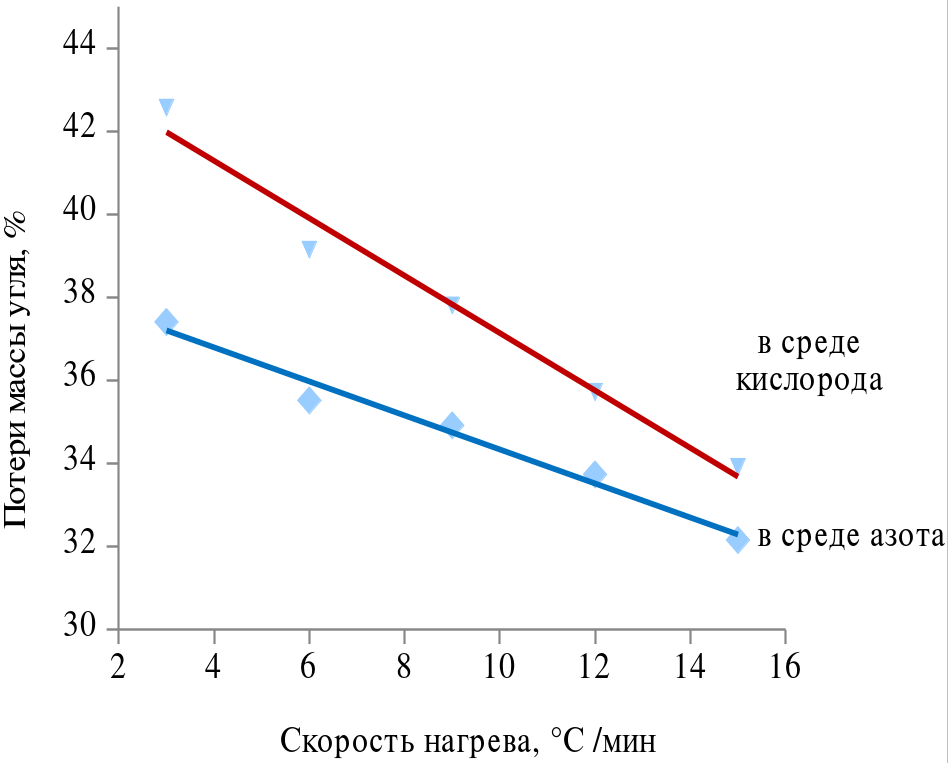
\includegraphics[width=0.5\textwidth]{image66}
\caption{Значения потери масс образцов угля при скоростях нагрева\\
6-15 град/мин в средах азота и кислорода}
\end{figure}

\begin{multicols}{2}
Выявлено, что увеличение скорости нагрева β от 3 до 15 град/мин на всех
стадиях разложения ОМУ заметно повышает значения температуры
Т\textsubscript{max}, которая растет при переходе 1→2→3 стадий. Так, для
среды азота общие изменения Т\textsubscript{max} для 1-й стадии
ΔТ\textsubscript{max} = 81 °С, 2-й стадии ΔТ\textsubscript{max} = 97 °С,
3-й стадии ΔТ\textsubscript{max} = 159 °С. Для среды кислорода общие
изменения Т\textsubscript{max} для 1-й стадии ΔТ\textsubscript{max} = 75
°С, 2-й стадии ΔТ\textsubscript{max} = 104 °С, 3-й стадии
ΔТ\textsubscript{max} = 134 °С (таблицы 2,3).

При увеличении скорости нагрева β от 3 до 15 град/мин повышается
скорость v\textsubscript{max} деструкции (соответствующие максимумам
основного разложения на дифференциальных кривых DTG), а также
наблюдается снижение активационного барьера процесса. С повышением
температуры при переходе от одной стадии основного разложения к другой
(на всем диапазоне изменения скорости нагрева) наблюдается заметное
увеличение Е\textsubscript{акт} , как в среде азота, так и кислорода.

Полученные значения показателей степени процесса \emph{n} (≈1,0-1,2)
показывают, что в силу многообразия и сложности физико-химических
превращений полученные кинетические параметры описывают не определенные
реакции, а суммарные процессы термического разложения ОМУ, и как выше
отмечалось, описывают только процесс основного термического разложения
ОМУ. Поэтому такие параметры можно рассматривать как «эффективные
параметры» формальной кинетики. Множество конкурирующих
последовательно-параллельных процессов при термодеструкции угля часто
приводит к колебаниям значения \emph{n} в интервале 0,5-1,5 {[}13{]}.

{\bfseries Выводы.} Таким образом, в работе исследована зависимость
кинетических характеристик термического разложения ОМУ от скорости и
температуры нагрева, описана зависимость между кинетическими параметрами
на разных стадиях основного разложения угля. Полученные данные
показывают, что более длительное время протекания термолиза оказывает
более существенное влияние на процесс деструкции угля, чем скорость его
нагрева. В целом можно отметить, что рассчитанные значения энергии
активации стадий основного термического разложения угля соизмеримы с
энергиями химических связей. Сам процесс основного термического
разложения ОМУ можно приближенно описать уравнением формальной кинетики
1-го порядка. Полученные результаты исследования могут быть применены
при определении режимов и ведении термохимических процессов разложения
углей, таких как газификация, коксование, полукоксование и др.
\end{multicols}

\begin{center}
{\bfseries Литература}
\end{center}

\begin{enumerate}
\item
Zhang Y., Li Y., Huang Y., Li S., Wang W. Characteristics of mass,
heat and gaseous products during coal spontaneous combustion using
TG/DSC--FTIR technology // Journal of Thermal Analysis and Calorimetry,
2019. -- P. 1-12.

\item
Худякова Г.И. Экспериментальное исследование термохимической
конверсии коксового остатка угля методом термогравиметрического анализа:
автореферат диссертации на соискание степени кандидата технических наук:
01.04.14, Екатеринбург, 2015. -- 24 с.

\item
Kosowska-Golachowska M. Thermal Analysis and Kinetics of Coal during
Oxy-Fuel Combustion // Journal of Thermal Science, 2017. -- Vol. 26. --
No. 4. -- P. 355-361.

\item
Su S, Pohl J.H., Holcombe D., Hart J.A. Techniques to determine
ignition, flame stability and burnout of blended coals in p.f. power
station boilers // Progress in Energy and Combustion Science, 2001. --
Vol. 27. -- P. 75-98.

\item
Jayaraman K., Kok M.V., Gokalp I. Thermogravimetric and mass
spectrometric (TG-MS) analysis and kinetics of coal-biomass blends //
Renewable energy, 2017. -- Vol. 101. -- P. 293-300.

\item
Wang G., Zhang J., Shao J., Liu Z., Zhang G., Xu T., Guo J., Wang H.,
Xu R., Lin H. Thermal behavior and kinetic analysis of co-combustion of
waste biomass/low rank coal blends // Energy Conversion and Management,
2016. -- V.124. -- P. 414-426.

\item
Das T., Baruah B.P., Saikia B.K. Thermal behaviour of low-rank Indian
coal fines agglomerated with an organic binder // Journal of Thermal
Analysis and Calorimetry, 2016. -- V.126. -- P.435-446.

\item
Лыгина Е.С., Дмитрук А.Ф., Галушко Л.Я., Любчик С.Б., Третьяков В.Ф.
Особенности изучения термодеструкции твердых и жидких органических
углесодержащих продуктов методом термогравиметрии // Химия твердого
топлива, 2009. -- № 3. -- С. 58-74.

\item
López F.A., El Hadad A.A., Alguacil F.G., Centeno T.A., Lobato B.
Kinetics of the Thermal Degradation of Granulated Scrap Tyres: A
Model-free Analysis // Materials Science, 2013. -- Vol. 19. -- No. 4. --
P. 403-408.

\item
Starink M.J. The determination of activation energy from linear
heating rate experiments: a comparison of the accuracy of isoconversion
methods // Termochimica Acta, 2003. -- Vol. 404. -- P. 163-176.

\item
Vyazovkin S., Burnhamb A.K., Criadoc J.M., Pérez-Maquedac L.A.,
Popescud C., Sbirrazzuolie N. ICTAC Kinetics Committee recommendations
for performing kinetic computations on thermal analysis data //
Thermocimica Acta, 2017. -- Vol. 505. -- P. 1-19.

\item
Бойко Е.А., Страшников А.В. Теоретическое обобщение и развитие
математического аппарата неизотермической кинетики // Известия РАН.
Энергетика, 2021. -- № 2. -- С. 97--118.

\item
Гюльмалиев А.М., Головин Г.С., Гладун Т.Г. Теоретические основы
химии угля. -- М.: Издательство Московского государственного горного
университета, 2003. -- 556 с.
\end{enumerate}

\begin{center}
{\bfseries References}
\end{center}

\begin{enumerate}
\item
Zhang Y., Li Y., Huang Y., Li S., Wang W. Characteristics of mass,
heat and gaseous products during coal spontaneous combustion using
TG/DSC--FTIR technology // Journal of Thermal Analysis and Calorimetry,
2019. -- P. 1-12.

\item
Khudyakova G.I. Experimental study of the thermochemical conversion
of the coke residue of coal by the method of thermogravimetric analysis:
abstract of the dissertation for the degree of candidate of technical
sciences: 01.04.14, Yekaterinburg, 2015. - 24 p.

\item
Kosowska-Golachowska M. Thermal Analysis and Kinetics of Coal during
Oxy-Fuel Combustion // Journal of Thermal Science, 2017. -- Vol. 26. --
No. 4. -- P. 355-361.

\item
Su S, Pohl J.H., Holcombe D., Hart J.A. Techniques to determine
ignition, flame stability and burnout of blended coals in p.f. power
station boilers // Progress in Energy and Combustion Science, 2001. --
Vol. 27. -- P. 75-98.

\item
Jayaraman K., Kok M.V., Gokalp I. Thermogravimetric and mass
spectrometric (TG-MS) analysis and kinetics of coal-biomass blends //
Renewable energy, 2017. -- Vol. 101. -- P. 293-300.

\item
Wang G., Zhang J., Shao J., Liu Z., Zhang G., Xu T., Guo J., Wang H.,
Xu R., Lin H. Thermal behavior and kinetic analysis of co-combustion of
waste biomass/low rank coal blends // Energy Conversion and Management,
2016. -- V.124. -- P. 414-426.

\item
Das T., Baruah B.P., Saikia B.K. Thermal behaviour of low-rank Indian
coal fines agglomerated with an organic binder // Journal of Thermal
Analysis and Calorimetry, 2016. -- V.126. -- P.435-446.

\item
Lygina E.S., Dmitruk A.F., Galushko L.Ya., Lyubchik S.B., Tretyakov
V.F. Features of the study of thermal destruction of solid and liquid
organic carbon-containing products by thermogravimetry // Chemistry of
solid fuels, 2009. - No. 3. - P. 58-74.

\item
López F.A., El Hadad A.A., Alguacil F.G., Centeno T.A., Lobato B.
Kinetics of the Thermal Degradation of Granulated Scrap Tyres: A
Model-free Analysis // Materials Science, 2013. -- Vol. 19. -- No. 4. --
P. 403-408.

\item
Starink M.J. The determination of activation energy from linear
heating rate experiments: a comparison of the accuracy of isoconversion
methods // Termochimica Acta, 2003. -- Vol. 404. -- P. 163-176.

\item
Vyazovkin S., Burnhamb A.K., Criadoc J.M., Pérez-Maquedac L.A.,
Popescud C., Sbirrazzuolie N. ICTAC Kinetics Committee recommendations
for performing kinetic computations on thermal analysis data //
Thermocimica Acta, 2017. -- Vol. 505. -- P. 1-19.

\item
Boyko E.A., Strashnikov A.V. Theoretical generalization and
development of the mathematical apparatus of non-isothermal kinetics //
Izvestiya RAN. Energy, 2021. - No. 2. - P. 97--118.

\item
Gyulmaliev A.M., Golovin G.S., Gladun T.G. Theoretical foundations
of coal chemistry. - M.: Publishing house of the Moscow State Mining
University, 2003. - 556 p.
\end{enumerate}

\begin{center}
\emph{{\bfseries Сведения об авторах}}
\end{center}

\begin{itemize}
\item
Нургалиев Нуркен Утеуович − кандидат химических наук, ассоциированный
профессор, кафедра «Химия, химическая технология и экология», Казахский
университет технологии и бизнеса, Республика Казахстан, г. Астана,
e-mail:
\href{mailto:nurgaliev_nao@mail.ru}{\nolinkurl{nurgaliev\_nao@mail.ru}}.

\item
Такирова Айгерим Хасеновна − магистр, старший преподаватель, кафедра
«Химия, химическая технология и экология», Казахский университет
технологии и бизнеса, Республика Казахстан, г. Астана, e-mail:
\href{mailto:adem_1996@mail.ru}{\nolinkurl{adem\_1996@mail.ru}}.

\item
Хамит Айтолкын Жумабаевна, магистр, старший преподаватель, кафедра
«Химия, химическая технология и экология», Казахский университет
технологии и бизнеса, Республика Казахстан, г. Астана, e-mail:
\href{mailto:aytolkyn.khamit-76@mail.ru}{\nolinkurl{aytolkyn.khamit-76@mail.ru}}.

\item
Жунусова Эльвира Бактыгалиевна, кандидат технических наук,
ассоциированный профессор, кафедра «Химия, химическая технология и
экология», Казахский университет технологии и бизнеса, Республика
Казахстан, г. Астана, e-mail:
\href{mailto:tahmina.66@mail.ru}{\nolinkurl{tahmina.66@mail.ru}}.

\item
Ахаева Айнур Акимхановна - магистр, старший преподаватель, кафедра
«Химия, химическая технология и экология», Казахский университет
технологии и бизнеса, Республика Казахстан, г. Астана, e-mail:
ainur\_akhaeva@mail.ru.
\end{itemize}

\begin{center}
\emph{{\bfseries Information about the authors}}
\end{center}

\begin{itemize}
\item
Nurgaliyev Nurken Uteuovich − Candidate of Chemical Science, Associate
Professor, Department of Chemistry, Chemical Technology and Ecology,
Kazakh University of Technology and Business, Republic of Kazakhstan,
Astana, e-mail:
\href{mailto:nurgaliev_nao@mail.ru}{\nolinkurl{nurgaliev\_nao@mail.ru}}.

\item
Takirova Aygerim Khasenovna - Master\textquotesingle s degree, senior
lecturer, Department of Chemistry, Chemical Technology and Ecology,
Kazakh University of Technology and Business, Republic of Kazakhstan,
Astana, e-mail:
\href{mailto:adem_1996@mail.ru}{\nolinkurl{adem\_1996@mail.ru}}.

\item
Khamit Aitolkyn Zhumabaevna, Master\textquotesingle s degree, senior
lecturer, Department of Chemistry, Chemical Technology and Ecology,
Kazakh University of Technology and Business, Republic of Kazakhstan,
Astana, e-mail:
\href{mailto:aytolkyn.khamit-76@mail.ru}{\nolinkurl{aytolkyn.khamit-76@mail.ru}}.

\item
Zhunussova Elvira Baktygalievna, Candidate of technical sciences,
Associate Professor, Department of Chemistry, Chemical Technology and
Ecology, Kazakh University of Technology and Business, Republic of
Kazakhstan, Astana, e-mail:
\href{mailto:tahmina.66@mail.ru}{\nolinkurl{tahmina.66@mail.ru}}.

\item
Akhaeva Ainur Akimkhanovna, Master\textquotesingle s degree, senior
lecturer, Department of Chemistry, Chemical Technology and Ecology,
Kazakh University of Technology and Business, Republic of Kazakhstan,
Astana, e-mail: ainur\_akhaeva@mail.ru.
\end{itemize}
